\chapter{El Proyecto}


\section{Motivación}

En la actualidad existen pocos sistemas Aplicados en el ámbito de la gestión en el area de medicina y los existentes suelen ser solo para áreas especificas


\section{Descripción del Proyecto}

Lo que se pretendió con este proyecto era poder desarrollar un sistema que unifique la areas de gestión y asignación de turnos y el manejo de historia clínica en un único sistema.

Cabe aclarar que el mismo se desarrollo con el propósito de poder ser utilizado principalmente en poli consultorios médicos ya que no plantea cuestiones tales como internaciones, traslado de pacientes, etc. como para poder ser de correcta utilidad en clínicas y hospitales. 


\section{Arquitectura de la Aplicación}

Implementado en Python utilizando en Framework Django, utilizando el motor de bases de datos PosgreSQL, funciona con una interfaz web por lo que se accede al mismo mediante un Navegador Web, Internamente maneja 2 módulos principales que son el  ``Modulo de Gestión de Turnos" y el ``Modulo de manejo de
Historia Clínica", al ser un sistema web implementa un tercer modulo de manera implícita que control de acceso mediante la definición de Grupos Usuarios y sus correspondientes permisos.


\section{Modulo Usuarios}

La gestión de usuarios es un proceso bastante común en casi todos los sistemas, muchos desarrolladores terminan programando funcionalidades de autenticación una y otra ves a lo largo de los a\'nos y casi siempre funcionando de la misma manera. Django se pensó para simplificar la vida no para complicarla, por eso
al ser una tarea bastante común en casi todas las aplicaciones, viene incluido un completo sistema de autenticación que gestiona:

\begin{itemize}
    \item Usuarios
    \item Grupos
    \item Permisos
    \item Sessiones de Usuarios y Cookies
\end{itemize}

Aunque en cuanto a lo que se refiere manejo de sesiones es un completo sistema solo maneja un pequeño conjunto de datos por lo que hubo que extender mediante la adición de un Modelo adicional para complementar la información de los usuarios.


\subsection{Modelos}

Aquí un diagrama con todos los modelos que componen el modulo Usuarios el cual está integrado en parte con el modulo Gestión de Turnos. Los Diagramas utilizados no corresponden a ninguna notación en particular solo sirven para mostrar la interacción en las diferentes clases, por lo que los modelos quizás se aproximen mas a una notación de Diagramas de clases en UML\footnote{UML o Proceso Unificado de Desarrollo de Software es una metodología de desarrollo que proporciona diferentes herramientas una de ellas es el diagrama de clases.} que la típica definición del DER \footnote{El DER o Diagrama Entidad Relacional el cual se usa para mostrar la interacción y cardinalidad entre las tablas de una base de datos.} aunque internamente se trabaje con un motor SQL (podrías usar un motor de bases de datos NoSQL)  y no con clases el uso de un determinado motor de base de datos será transparente para el usuario no se necesitara modificar más que la configuración de la aplicación el resto seguirá como si nunca lo hubieses notado. \footnote{A lo sumo elegiremos entre uno y otro motor de bases de datos por una cuestión de performance más que nada.}

\begin{figure}[H]
    \centering
    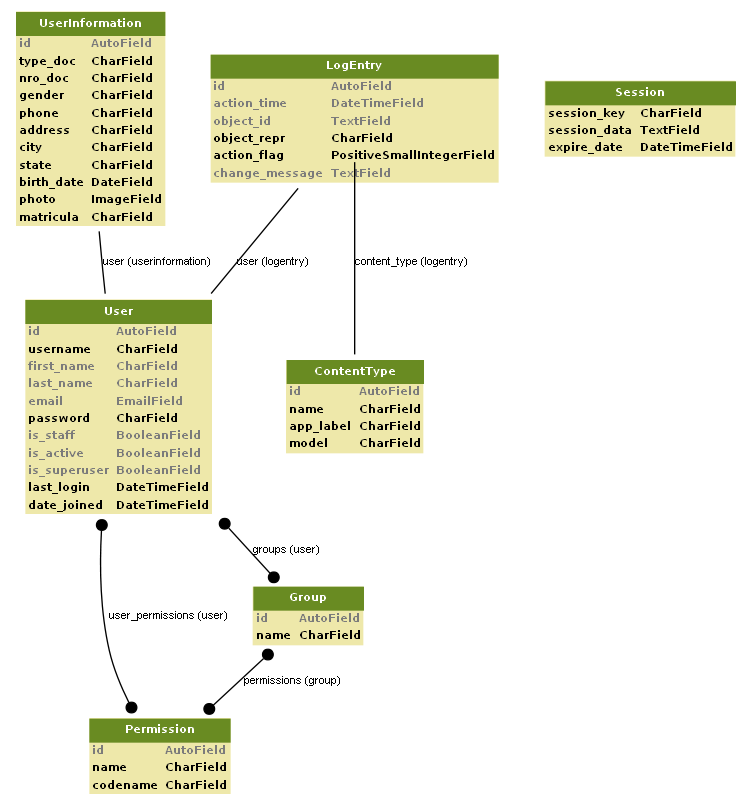
\includegraphics[scale=0.45]{resourse/auth.png}
    \caption{Diagrama con modelos que componen el modulo Usuarios}
    \label{fig:07}
\end{figure}

El único modelo que fue necesario agregar es \textbf{UserInformation} que es para extender la información que se registra en el modelo \textbf{User} el resto vienen con Django. En Resumen aunque se podría haber desarrollado Un Modulo desde cero que gestione las sesiones de usuarios hubiese generado trabajo extra sin sentido.

\subsection{Usuarios y Permisos}

El sistema contempla 4 tipos de usuarios los cuales son: 

\begin{itemize}
    \item Usuarios no registrados 
    \item Pacientes
    \item Médicos
    \item Administrativos
\end{itemize}

\subsubsection{Usuarios no Registrados}

Los \textbf{Usuarios no registrados} que vendría a ser cuando el usuario ingresa a la aplicación y no hay ninguna sesión iniciada, pueden acceder al sistema para consultar información básica y horarios de atención de los especialistas que forman parte de la institución, además de tener la opción de registrarse como paciente.\\[0.1cm]    

\subsubsection{Paciente}

El rol \textbf{Paciente} corresponde a los usuarios comunes, un usuario paciente puede ser creado por cualquiera de los otros roles, en caso que sea un usuario no registrado quien da el alta como paciente, el mismo deberá confirmar el registro mediante un código de verificación que el sistema le enviara al correo antes de poder comenzar a usar su cuenta, en los otros casos (el usuario Paciente es registrado por un 
medico o un Administrativo) no se requerida dicha confirmación.\\[0.1cm]

En cuanto a los privilegios del usuario Paciente, este además de poder consultar la  información de los especialistas puede solicitar un turno para ser atendido a un especialista en particular, también realizarle una interconsulta (mediante el sistema interno de mensajería) y modificar sus datos básicos, en resumen sus posibles funciones son:


\subsubsection{Medico}

Los Usuarios \textbf{Médicos} los cuales son asignados por los Administrativos a los Especialistas, en cuanto a privilegios y funcionalidades dentro del sistema, los mismos pueden:

\begin{itemize}
    \item Registrar Pacientes
    \item Modificar datos de Pacientes
    \item Enviar Mensajes a cualquier Usuario
    \item Registrar Turnos 
    \item Cancelar Turnos
    \item Administrar sus Horario de Atención
    \item Cancelar días de atención
\end{itemize}

Son los únicos usuarios que tienen acceso al Modulo \textit{Historia Clínica}, en cuanto a privilegio sobre este modulo diremos que tiene la posibilidad de Crear, Modificar, Borrar (salvo casos específicos, que por su naturaleza no se permite dicha modificación.) un conjunto de Estudios, para más detalle se recomienda consultar el apartado sobre tal modulo.


\subsubsection{Administrativo}

En cuanto a los usuarios \textbf{Administrativo} poseen los mismos permisos que un usuario \textbf{Medico} exceptuando que no poseen acceso a las funcionalidades del Modulo Historia Clínica, como privilegio especial pueden administrar las cuentas de usuario de todos los roles incluidos en el sistema, incluido los 
Medico y otros Administrativos.

\subsubsection{Admin}

Existe un rol adicional que Django crea y gestiona por aparte, el mismo queda delegado para los administradores del sistemas ya que mediante el se puede acceder y modificar cualquier parte de la base de datos, por lo que podríamos decir que es un \textbf{Súper Usuario}, o usuario \textbf{Root} como para hacer analogía con los usuarios en entornos Unix, el mismo no forma parte del sistema desarrollado sino como funcionalidad adicional Django provee un panel de administración, para dicho tipo de usuario, al cual se puede acceder desde \url{/admin/} por ejemplo si estuviésemos ejecutando en un servidor local la ruta completa seria \url{http://127.0.0.1/admin/}\footnote{Se puede consultar mas acerca de Django
Admin en \url{https://docs.djangoproject.com/en/dev/ref/contrib/admin/}}.\\[0.1cm]


\begin{figure}[h]
    \centering
    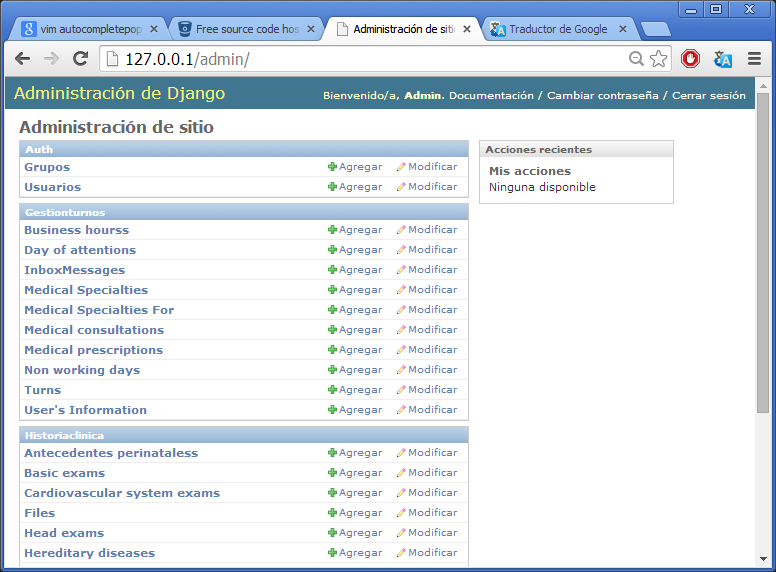
\includegraphics[scale=0.5]{resourse/django-admin.png}
    \caption{Vista del Panel Administracion provisto por Django}
    \label{fig:123}
\end{figure}  


Cabe aclarar que el Súper Usuario del sistema de autenticación de Django dentro del sistema en sí mismo no posee ningún privilegio adicional, es mas para compatibilizar el usuario con la funcionalidad del sistema, cuando se inicializan por primera vez, se crea un usuario de este tipo llamado \textbf{admin}\footnote{Se debe crear con ese nombre de usuario para evitar problemas en la inicialización, después se puede eliminar si se desea el usuario.} al cual se le asignan privilegio de \textit{Administrativo}.


%%%%%%%%%%%%%%%%%%%%%%%%%%%%%%%%%%%%%%%%%%%%%%%%%%%%%%%%%%%%%%%%%%%%%%%%%%%%%%%

\section{Modulo Gestión de Turnos} 

Dejando de lado el modulo Usuarios que nos provee Django el sistema desarrollado se divide esencialmente en 2 partes o módulos, aquí explicare como se diseño e implemento el Modulo Gestión de Turnos, que a mi consideración fue el que mayor reto aporto a la hora de pensar un solución para poder implementarlo.

El modulo se encarga de implementar las siguientes funciones

\begin{itemize}
    \item Gestionar Datos de Usuarios
    \item Mensajería Interna
    \item Asignación de Especialidades Medicas
    \item Asignación de Turnos
\end{itemize}


\subsection{Definición del Modelo}

Aquí se muestra el diagrama de modelos que componen el modulo \textbf{Gestión de Turnos} \footnote{Vuelven a aparecen los modelos \textbf{User} y \textbf{UserInformation} por que casi todos los otros modelos dependen de alguna forma de ellos}, por la cantidad de modelos se mostrara en 2 diagramas, igualmente téngase en cuenta que corresponden a un único modelo, lo que haremos será separar en los modelos específicos utilizados para gestión de turnos y el resto de los modelos definidos que complementan la funcionalidad del modulo.


\subsection{Gestionar Datos de Usuarios}

Esta funcionalidad describe, todo lo referido en cuanto al alta, baja y modificación de los datos de todos los usuarios. Implementa la vista tanto para modificación de datos personales, vistas de administrador para gestionar datos de otros usuarios. 


\subsection{Mensajería Interna}

Permite la comunicación interna entre los usuarios, su principal utilidad es permitir que los Pacientes puedan realizar pequeñas interconsultas a los médicos atraves de la plataforma, sin requerir una consulta médica.

\subsection{Asignación Especialidades Medicas}

Dentro el modulo permite asignarles especialidades medicas correspondientes a los profesionales, aunque no realiza una distinción especifica a la hora de asignar turnos, simplemente considera que el médico en dicho horario puede atender cualquier consulta relacionada a sus especializaciones. \footnote{Tengase en cuenta que es raro ver un medico con varias especializaciones medicas y que el sistema fue pensado para ser utilizado en un consultorio médico, donde no se suele contar con equipamiento de alta complejidad.}


\subsection{Asignación de Turnos}  

La \textit{Asignación de Turnos} a los pacientes es la principal funcionalidad del modulo, que entre otras funcionalidades permite:

\begin{itemize}
    \item Definir días de atención
    \item Definir días feriados o de Vacaciones     
    \item Asignar turnos
    \item Controlar la asistencia de los pacientes.    
\end{itemize}

Por Cuestiones de tamaño del diagrama y por la cantidad modelos utilizados en el modulo se complicaba poder mostrarlos todo en una misma página por lo que para mejor visualización e interpretación separe el mismo en 2 partes:

El primer diagrama unifica todo lo referente a la asignación de turnos, que es lo principal del modulo:

\begin{figure}[H]
    \centering
    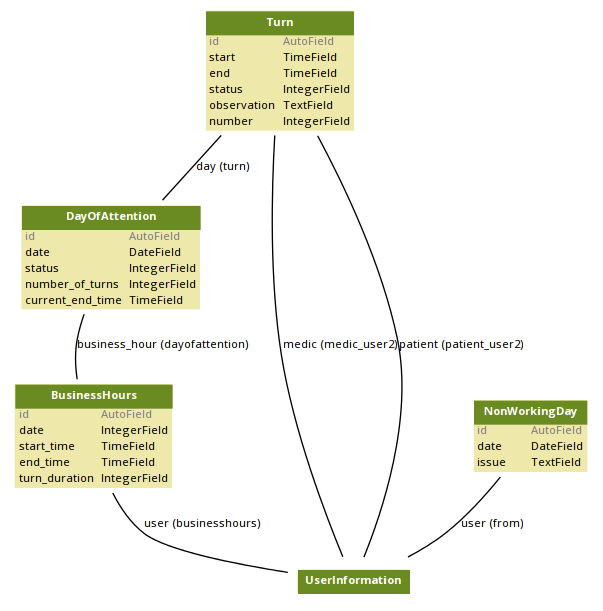
\includegraphics[scale=0.6]{resourse/gt-gt.png}
    \caption{Modulo Gestion Turnos - Diagrama Modelos correspondiente a la Gestión de Turnos}
    \label{fig:124}
\end{figure}  

En el segundo diagrama se muestra los modelos necesarios para las funcionalidades adicionales.

\begin{figure}[H]
    \centering
    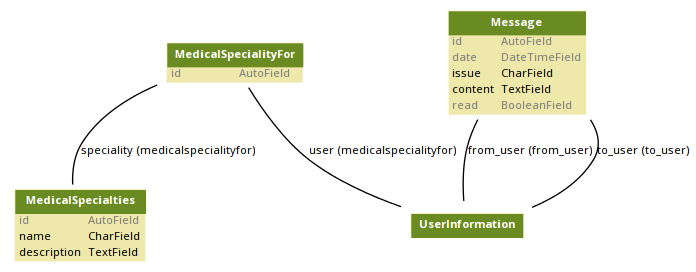
\includegraphics[scale=0.6]{resourse/gt-ot.png}
    \caption{Modulo Gestión Turnos - Modelos Adicionales}
    \label{fig:125}
\end{figure}  


%\\[0.5cm]

\subsection{Diseño de Modelos Para la Gestión de Turnos}

Aqui se muestran los algunas consideraciones que se tuvieron en cuenta a la hora de diseñar los modelos para implementar la funcionalidad de asignación de turnos propiamente dicha la cual define el nombre del modulo. 


\subsubsection{BussinesHour(Horario De Atención)}

Este modelo se utiliza para definir el horario de atención de cada médico, en el se especifican parámetros como:

\begin{itemize}
    \item \textbf{user}: referencia al médico al cual pertenece 
    \item \textbf{date}: define el día de atención \footnote{Esto hace  referencia a los días de la semana ósea Lunes, Martes,..., etc. por el momento solo se puede definir un único día de atención por día por medico.}
    \item \textbf{start\_time, end\_time}: marcan el horario de inicio y fin del  día de atención del médico.
    \item \textbf{turn\_duration} duración estimada del turno en minutos.
\end{itemize}

En base a esto se puede calcular un dato adicional que es la cantidad de turnos que se pueden asignar en tal día, y se hace de la siguiente manera:

\begin{lstlisting}
numero\_turnos = (hora\_fin - hora\_inicio) // turn\_duration
\end{lstlisting}

Esto devolverá un valor entero por truncamiento, que será el numero máximo de turnos que se puedan asignar.


\subsubsection{DayOffAttention (Días de Atención)}

Este modelo maneja la disposición horaria de una fecha en particular, se basa en los datos que se definieron en el modelo anterior \textbf{BussinesHour}, por lo que solo se pueden generar en las fechas que correspondan con los días de la semana asignados, cuenta con los siguientes parámetros:

\begin{itemize}
    \item \textbf{bussines\_hour}: referencia al horario de atención definido  por el médico.
    \item \textbf{date}: qué fecha cae ese día, esto se refiere al día del año  especifico.
    \item \textbf{status}: información del estado del día, es de tipo booleano  y especifica el estado del día de atención siendo el valor TRUE para explicar que se pueden asignar más turnos y FALSE que no se  pueden asignar más. \footnote{ Que un día de atención este marcado como no disponible (status=FALSE) puede significar que el cupo este lleno o que ese día el médico no pueda asistir o sea feriado por ejemplo, para         determinar de qué se trata si dice no disponible y no hay ningún turno asignado (number\_of\_turns=0) significara que ese día el médico no atiende }
     \item \textbf{number\_of\_turns}: numero de turnos que van siendo asignados
     \item \textbf{current\_end\_time}: horario actual de finalización 
\end{itemize}


\subsubsection{Turn (Turno)}

Este modelo se define para registrar la información correspondiente a los turnos asignados es dependiente del modelo anterior \textbf{DayOffAttention} donde se especifican el resto de los datos como la fecha.

En cuanto a sus atributos, mucho no hay que explicar y son:

\begin{itemize}
    \item \textbf{day}: hace referencia a un día de atención (DayOffAttention)
    \item \textbf{medic}: referencia a los datos del médicos
    \item \textbf{patient}: referencia al paciente. 
    \item \textbf{start, end}: hacen referencia a las horas de inicio y fin correspondientemente.
    \item \textbf{status}: estado del turno es de tipo enumerado define varios posibles estados entre los que están (pendiente, concretado, cancelado medico, cancelado paciente).
    \item \textbf{observation}: campo de texto, para registrar cualquier  observación pertinente.
    \item \textbf{number}: se refiere al número de orden para atención.
\end{itemize}


\subsubsection{Consideraciones}

En cuanto a funcionamiento de la asignación de turnos se tienen en cuenta las siguientes consideraciones: \\[0.1cm]

Un turno no puede ser cancelado después de su hora de inicio por el paciente, siendo así posible de ser cancelado por el médico. \\[0.1cm]

Al ser cancelado por un paciente se debe cambiar correspondiente estado dentro de día de atención. \\[0.1cm]

 Si un medico cancela un turno el mismo no se modificara el estado en la tabla  día de atención, como el caso de los paciente que cancelen un turno, para el sistema hará de cuenta que los mismo ocurrieron, aunque si un turno es cancelado por el médico el mismo no será reprogramado. \\[0.1cm]

 En todos los casos los usuarios deberían poder recibir el correspondiente notificación de que se cancelo dicho turno invitándolos a reprogramar el mismo. \\[0.1cm]

Los pacientes no pueden solicitar turnos durante el horario de atención del mismo, si el servidor comprueba que existen turnos sin actualizar estado como pendientes, si el médico o administrador no actualizo los mismos y ya paso la hora del mismo tiene que enviar notificaciones correspondientes. \\[0.1cm]


%%%%%%%%%%%%%%%%%%%%%%%%%%%%%%%%%%%%%%%%%%%%%%%%%%%%%%%%%%%%%%%%%%%%%%%%%%%%%%

\section{Modulo Historia Clínica}

Este modulo del sistema tiene como tarea manejar y recolectar toda información referente a las historia clínica de los pacientes.


\subsection{¿Que es una Historia Clínica?}

Antes de entrar en todo lo referente sobre el desarrollo del correspondiente modulo tomo un momento para explicar concretamente a que no referimos cuando hablamos de la misma por lo que aquí tenemos la siguiente definición:

La historia clínica es un documento médico-legal que surge del contacto entre el profesional de la salud (médico, podólogo, psicólogo, asistente social, enfermero, kinesiólogo, odontólogo, etc.) y el paciente donde se recoge la información necesaria para la correcta atención de los pacientes. La historia clínica es un documento válido desde el punto de vista clínico y legal, que recoge información de tipo asistencial, preventivo y social.

La Historia Clínica se origina con el primer episodio de enfermedad o control de salud en el que se atiende al paciente, ya sea en el hospital o en el centro de atención primaria, o en un consultorio médico. La historia clínica está incluida dentro del campo de la semiología clínica \footnote{La Semiología Clínica es el cuerpo del conocimiento que se ocupa de la identificación de las diversas manifestaciones patológicas \cite{SemiClin}}.

\subsection{La Historia Clínica en la Ley Argentina}

La documentación médica comprendida en lo que comúnmente se denomina ``historia clínica" la cual no se encontraba regida por leyes especificas en la Argentina hasta el 19 de noviembre del 2009 donde se promulga la Ley 26.529 \cite{LeyHC}.\\[0.1cm]

En el capítulo primero de la ley se enumeran los derechos de los pacientes, en el artículo 2, inciso ``a". Renueva el derecho a la intimidad y la confidencialidad, donde se hace hincapié sobre la responsabilidad de preservar la intimidad y confidencialidad de toda la documentación médica concerniente a los pacientes, particularmente el inciso ``d" del mismo artículo:\\[0.1cm]

``El paciente tiene derecho a que toda persona que participe en la elaboración o manipulación de la documentación clínica, o bien tenga acceso al contenido de la misma, guarde la debida reserva, salvo expresa disposición en contrario emanada de autoridad judicial competente o autorización del propio paciente".\\[0.1cm]

Garantiza además el respeto por la autonomía del paciente y el derecho a recibir la información necesaria para su salud, incluyendo el derecho a negarse a ser informado.\\[0.1cm]

El capítulo III reza sobre el Consentimiento Informado, el cual está basado en el principio de autonomía, es decir, el derecho del paciente a ser reconocido como persona libre y dueña de tomar sus decisiones. Para ello el paciente debe estar en condiciones de comunicar su decisión y  éste ha sido informado adecuadamente de 
sus opciones, es decir, no pueden ser decisiones hechas como resultado de delirio o alucinaciones. La decisión del paciente es consistente con sus valores y metas y se mantiene estable en el tiempo si no han habido modificaciones hechas por el mismo sujeto. Los familiares de un paciente no están en el derecho de 
requerir al médico del paciente que no se le comunique ciertos detalles o información al mismo. \\[0.1cm]

Ahora bien vallamos a lo que nos interesa:\\[0.1cm]

La ley define a la Historia Clínica como el documento ``obligatorio, cronológico,\footnote{En este sentido la ley está un poco atrasada ya que no contemplaba en ese momento la informatización de la historia clínica.} foliado y completo en el que consta toda actuación realizada al paciente por profesionales y auxiliares de la salud." Define que la historia clínica es propiedad del paciente, siendo este el titular de la misma. Siempre que un paciente solicite la historia clínica, la institución competente debe entregarle una copia autenticada en 48 horas. Si no es entregada en ese plazo, el paciente está autorizado a interponer un recurso de Habeas Data, juzgado de por medio. \\[0.1cm]

Entre los datos que han de consignarse en forma obligatoria esta la fecha de inicio y confección de la historia clínica, datos identificatorios del paciente y su núcleo familiar, datos del profesional interviniente y su especialidad, registros claros y precisos de los actos realizados por profesionales y auxiliares intervinientes, antecedentes genéticos, fisiológicos y patológicos si los hubiere, y todo acto médico realizado o indicado.\\[0.1cm]

Incluye en la historia clínica a todos los documentos que hagan referencia a  información de salud del paciente, añadiendo los consentimientos informados, hojas de indicaciones, hojas de enfermería, estudios complementarios,  incluyendo las ``prácticas realizadas, rechazadas o abandonadas." Esto  último es interesante: si el paciente abandona o rechaza un tratamiento propuesto, es responsabilidad del médico consignarlo, que a fin de cuentas es el beneficiario de que aquello quede asentado desde el punto de vista médico-legal.\\[0.1cm]

Autoriza a reclamar una copia de la historia clínica al paciente y su representante legal, al cónyuge o conviviente de hecho (sin importar el sexo), y a los herederos forzosos. Lo que no queda claro del art. 19 inciso b es si los cónyuges y convivientes requieren o no la autorización del paciente.\\[0.1cm]

Se añade esta ley al capítulo 11 del Código de ética de la Asociación Médica Argentina, del año 2001. En ella se explaya en forma más extensa y detallada sobre la confección. Particular interés debiéramos prestarle al art. 168:\\[0.1cm]

``La historia clínica ha de ser un instrumento objetivo y comprensible por terceros, y no solo por quienes escriben en ella." A su vez, el art. 171 especifica que "debe ser legible, no debe tener tachaduras, no se debe escribir sobre lo ya escrito, no debe ser borrada, no se debe dejar espacios en blanco y ante una equivocación debe escribirse ERROR y aclarar lo que sea necesario. No se debe añadir nada entre renglones. \footnote{Esto último es solo para la versión en papel}"


\subsection{Funcionalidades}

Las funcionalidades que se implementan en correspondiente módulos son solo básicas y comprenden la documentación practicas más comunes dentro del área de la medicina, esto no implica que solo valla a servir para eso únicamente, por su estructura el modulo contempla la posibilidad de agregar nuevos componentes para estudios específicos que sean requeridos y que no hayan sido contemplados en el actual sistema.\\[0.1cm]

El modulo se encarga básicamente de registrar los diferentes estudios que se le practican a un paciente, adicionalmente registra información correspondiente a las interconsultas \footnote{Consultas medicas realizadas por el paciente} y las observaciones del médico, así como los medicamentos que fueron recetados por el especialista.


\subsection{Definicion de Modelos}

Los modelos que componen el Modulo corresponden a los diferentes tipos de exámenes de practica mas común \footnote{Esto no es que este definido en algún lado que sean solo estos, sino que más bien son los exámenes que durante el análisis de diferentes modelos se presentaban mas comúnmente.} en lo que 
Corresponden a la historia clínica.\\[0.1cm]

Aquí también por la cantidad de modelos se hace difícil poder colocarlos todos en un único diagrama dentro de la pagina por lo que también se separara en varias partes sin romper las relaciones de los mismo, ósea aunque se realice una separación de los mismos corresponden a un único modulo por lo que tendrían que verse como un todo y no como partes separadas: \\[0.1cm]


\subsection{Modelos Básicos}

\begin{figure}[H]
    \centering
    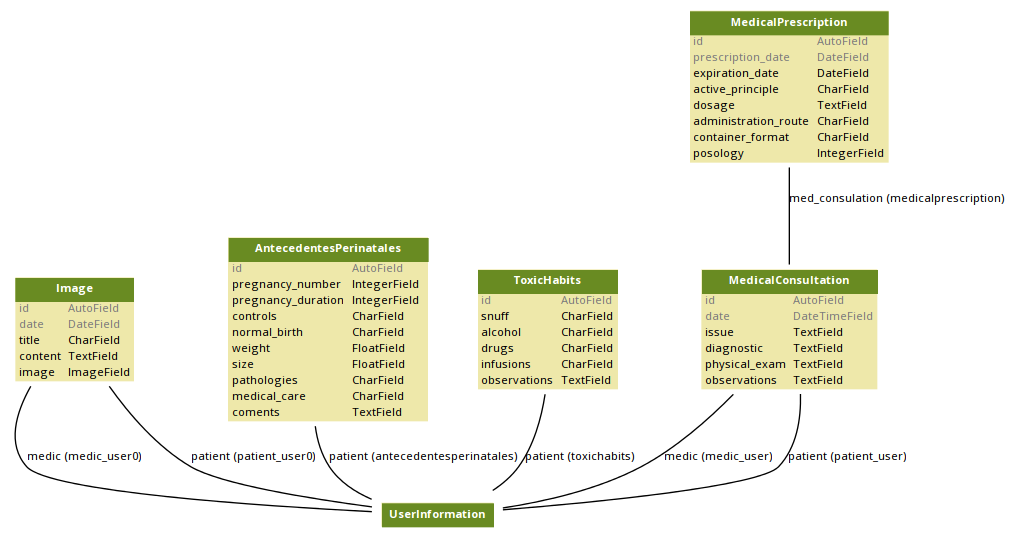
\includegraphics[scale=0.4]{resourse/hc1.png}
    \caption{Historia Clínica Modelos Básicos}
    \label{fig:hc3}
\end{figure} 

\subsubsection{Image}
Modelo encargado de almacenar imágenes de importancia sobre estudios realizados al paciente.

\begin{itemize}
    \item \textbf{title} titulo de la imagen
    \item \textbf{content} Información adicional sobre la imagen.
    \item \textbf{date} Fecha que se tomo la imagen
    \item \textbf{image} referencia al archivo 
\end{itemize}

\subsubsection{MedicalConsulation (Consulta Médica)}
Este Modelo almacena la información que el médico registra durante la consulta médica desde el motivo que origino la consulta, observaciones del médico, y demás datos de relevancia:

\begin{itemize}
    \item \textbf{date} Fecha de la consulta
    \item \textbf{issue} Motivo de la consulta
    \item \textbf{diagnostico} Diagnostico del medico.
    \item \textbf{physical\_exam} Observaciones del Examen Físico \footnote{Corresponde a un examen menor o visual simple que el médico realiza al paciente}
    \item \textbf{observations} Anotaciones Adicionales. 
\end{itemize}

\subsubsection{MedicalPrescription (Receta Médica)}

Almacena información relevante sobre el medicamento prescripto en la receta médica, como se observa en el modelo las recetas medicas dependen directamente de una consulta médica, se asume que no se puede recetar un medicamento sin existir una consulta médica previa, aunque a partir de una consulta médica, se pueden generar varias recetas. Los datos que almacena el modelo se corresponden según las normas actuales sobre información que debe contener una receta médica y son:

\begin{itemize}
    \item \textbf{prescription\_date} Fecha que fue prescripto el medicamento
    \item \textbf{expiration\_data} Vencimiento de la receta, pasada esta fecha la  misma debe considerarse invalida.
    \item \textbf{active\_principie} Principio Activo o nombre genérico de la monodroga que se receta.
    \item \textbf{dosage} Tamaño de la dosis
    \item \textbf{administration\_route} Modo en que se debe tomar la droga
    \item \textbf{container\_format} Formato del Envase y cantidad.
    \item \textbf{posology} Cada cuanto debe administrarse y porque periodo
\end{itemize}

\subsubsection{Antecedentes Perinatales}
Este tipo de modelo registra un único informe y se corresponde a los datos de nacimiento del paciente si es que existen, registra la siguiente información:

\begin{itemize}
    \item \textbf{pregnancy\_numbre} Numero de embarazo de la madre.
    \item \textbf{pregnacy\_duration} Duración del embarazo en semanas.
    \item \textbf{controls} Si asistió a controles médicos durante el embarazo.
    \item \textbf{normal\_birth} Nació de parto normal o por cesárea.
    \item \textbf{weight} Peso al nacer.
    \item \textbf{size} Tamaño al nacer.
    \item \textbf{pathologies} Presento complicaciones al nacer.
    \item \textbf{medical\_care} Requirió atención medica especial.
    \item \textbf{observations} Otras anotaciones.
\end{itemize}

\subsubsection{ToxicHabit (Hábitos Tóxicos del Paciente)} 

Se refiere a si el paciente consume algún tipo de droga ósea refleja las adicciones del mimo sin importar si las drogas son legales o ilegales, para ayudar a determinar posibles causas y complicaciones en su evolución.

\begin{itemize}
    \item \textbf{snuff} Tabaco
    \item \textbf{alcohol} Alcohol
    \item \textbf{drugs} Drogas
    \item \textbf{infusions} Infusiones
    \item \textbf{observations} Anotaciones Adicionales. 
\end{itemize}


\subsection{Modelos de los diferentes tipos de Examen}

En este caso no se entrara en detalle sobre los datos e información que se registra estos modelos por cuestiones de que la mismas escapan del conocimiento común de las personas, si desea saber más acerca de ello en la bibliografía están las documentación en base que datos o modelos se modelaron los exámenes.

\begin{figure}[H]
    \centering
    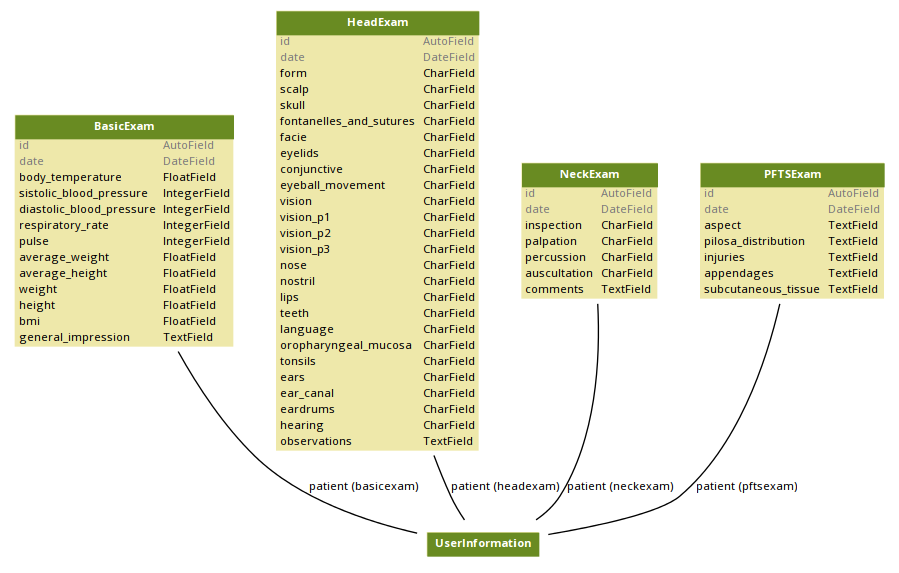
\includegraphics[scale=0.5]{resourse/hc3.png}
    \caption{Historia Clínica Modelos de Estudios}
    \label{fig:hc2}
\end{figure} 


\subsubsection{BasicExam (Examen Básico)}

El Modelo \textbf{BasicExam} refleja la información correspondiente a un examen físico general sin entrar en análisis de examen de espéciales de las diferentes áreas del cuerpo.


\subsubsection{HeadExam (Examen de Cabeza)}

Un xxamen más especializado de la cabeza,  en el que se analiza conjuntamente boca, ojos, nariz, forma del cráneo y oídos.


\subsubsection{NeckExam (Examen de cuello)}
Está orientada a buscar cambios en la forma del cuello (adenopatías, bocio, lipomas, quistes o tumores), en este caso es muy importante la ubicación del aumento de volumen cervical que oriente en el diagnostico.

\subsubsection{PFTSExam (Examen de Piel Faneras y Tejido Subcutáneo)}

Este modelo está orientado a registrar información correspondiente a estudio y descripción completa de: piel, faneras cutáneas, mucosas, tejido celular subcutáneo y músculos.

\begin{figure}[H]
    \centering
    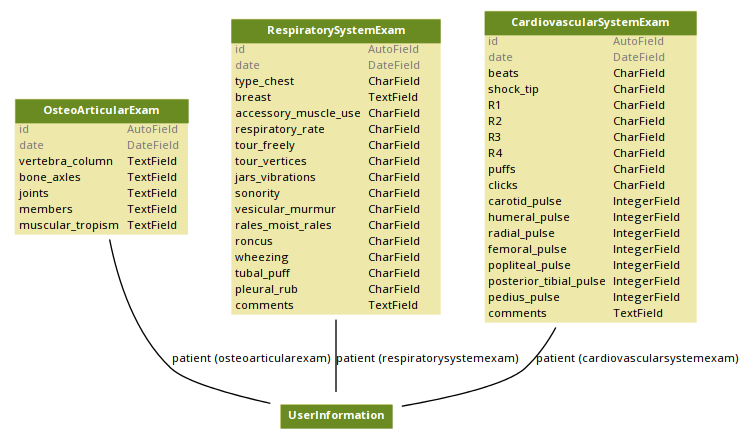
\includegraphics[scale=0.5]{resourse/hc4.png}
    \caption{Historia Clínica Modelos de Estudios Continuación}
    \label{fig:hc3}
\end{figure} 


\subsubsection{OsteoArticularExam (Examen Osteo Articular)}

El Examen Osteo Articular contempla la evaluación de la fuerza muscular esquelética medición de los miembros y movilidad Articular, en el se analizan la:

\begin{itemize}
    \item Simetria Estructural y Alineación
    \item Facilidad y Amplitud de Movimientos
    \item Masa y tono Muscular
    \item Fuerza Muscular
    \item Apariencia de la piel sobre las articulaciones.
    \item Dolores, crepitaciones y deformidades
\end{itemize}

\subsubsection{RespiratorySystemExam (Examen del Sistema Respiratorio)}

Consiste en un examen en el cual se analizan cada una de los componentes del sistema respiratorio, se analizan:

\begin{itemize}
    \item Tórax
    \item Sonoridad
    \item Capacidad Pulmonar
    \item Boca, fosas nasales, faringe, laringe y tráquea 
    \item Vías Aéreas
    \item Frecuencia Respiratoria
    \item Músculos Accesorios y Vesiculares
\end{itemize}

\subsubsection{CardiovascularSystemExam (Examen del Aparato Cardiovascular)}

Este análisis trata de almacenar lo referente al estudio del sistema cardiovascular el cual está constituido por el corazón y los vasos sanguíneos (arterias, capilares y venas) el análisis permite recoger información sobre:

\begin{itemize}
    \item Numero Latidos Por Minutos 
    \item Choques de Punta
    \item R1, R2, R3 y R4
    \item Murmullo Vesicular y Chasquidos
    \item Pulso Carotideo
    \item Pulso Humeral
    \item Pulso Radial
    \item Pulso Femoral
    \item Pulso Poplíteo
    \item Pulso Tibial Posterior
    \item Pulso Pedio
    \item Observaciones Generales
\end{itemize}


